\documentclass{article}

\usepackage{amsmath} % Required for some math elements 
\usepackage{natbib} % Required to change bibliography style to APA
\usepackage{siunitx} % Provides the \SI{}{} and \si{} command for typesetting SI units
\usepackage{subfigure}
\usepackage{graphicx}


\title{Answers to The Questions} 

\date{\today}

\begin{document}

\maketitle

\section{The Structure of our network}
Most time, we use 1-hidden-layer neural network with 300 units. Mathmatically, $y_{train} = W_2*h(W_1*a_0)$, where $a_0$ is the vectorized images and function $h$ is the active function. Here, we choose the ReLu function. i.e.
\begin{equation}
h(x) = \begin{cases}
x, & x>=0 \cr
0, & x<0 
\end{cases}
\end{equation}

For notations, we set $z_l = W_l * a_{l-1}$ and $a_l = h(z_l)$, where $l$ means the $l^{th}$  layer (in our network, $l$ can only be 1 or 2). We use $L$ to represent the last layer (in our network, $L$ = 2). \\

However, in section 2.2 "Comparison of different network structure", we modified the number of layers and units in each layer. [300] means 1 hidden layer with 300 units. [300,150] means 2 hidden layers and 300 units in the first layer and 150 units in the second layer. [150,300] means 2 hidden layers and 150 units in the first layer and 300 units in the second layer.\\
\\
Some parameters:\\
$\beta$: the weight before $z_l=W_l*a_{l-1}$ constraint.\\
$\gamma$: the weight before $a_l = h(z_l)$ constraint. \\
$\lambda$: the Lagrange multiplier term. \\
$\epsilon$: a constant that initialize $W$, $z$ and $a$.\\
In our program, we initialized $W_l = \epsilon*randn(sizeof(W_l))$, $z_l = \epsilon*randn(sizeof(z_l))$  and $a_l = \epsilon*randn(sizeof(a_l))$.

\section{Explaination about $\epsilon$}
In the paper, they mentioned that $a$ and $z$ should be initialized with normal distribution.
We got this initializing method from the open course "CS231n Convolutional Neural Networks for Visual Recognition"of Stanford University.
Interestingly, as showed in the next section, when $\epsilon$ is 1, all the energies will go down but the accuracy is lower. While $\epsilon$ is 0.0001, one of the energies will go up but the accuracy is higher. We found this result yesterday and haven't got any thinking about this.

\section{Energy}
As our network has 1hidden-layer, we plotted the energy of $||z_1 - W_1*a_0||^2$, $||z_2 - W_2*a_1||^2$ and loss energy which is softmax here.
Here are the results.
\begin{figure}[htbp]
\centering
\subfigure[loss energy]{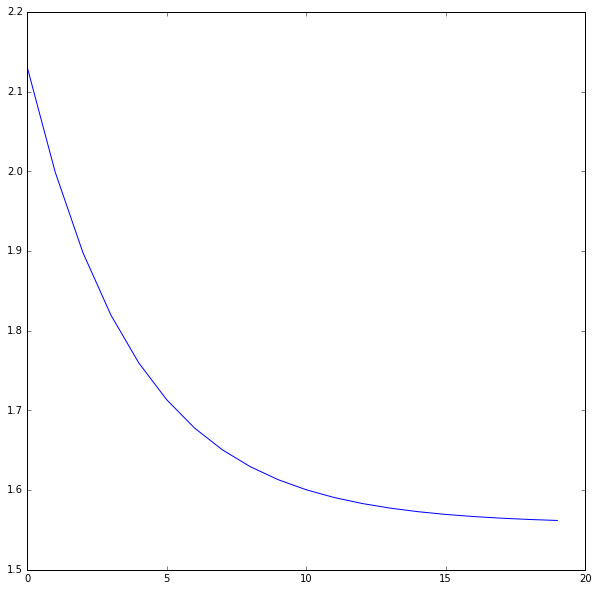
\includegraphics[scale=0.15]{1_dataloss.png}}
\subfigure[$||z_1 - W_1*a_0||^2$]{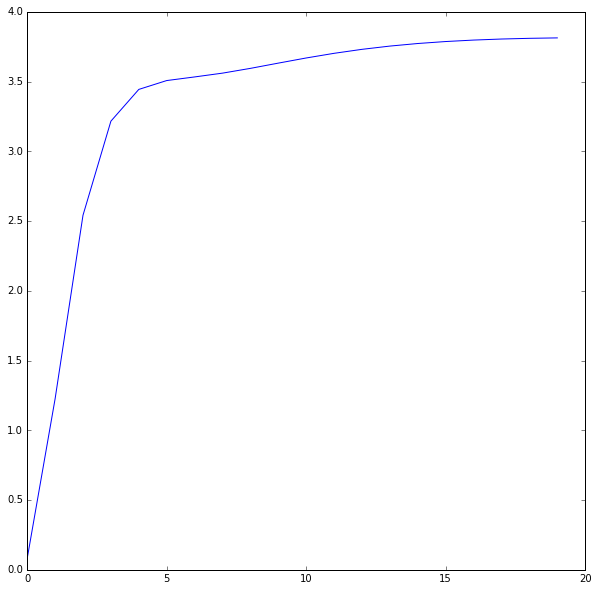
\includegraphics[scale=0.15]{1_qudraloss0-1.png}}
\subfigure[$||z_2 - W_2*a_1||^2$ ]{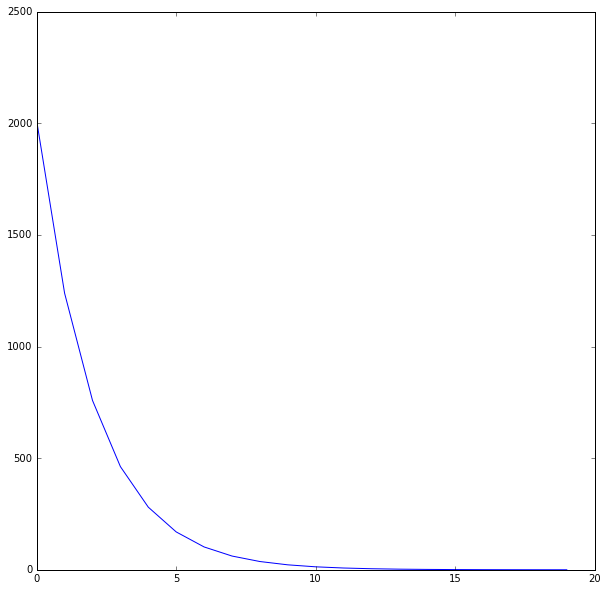
\includegraphics[scale=0.15]{1_qudraloss1-2.png}}
\subfigure[loss energy]{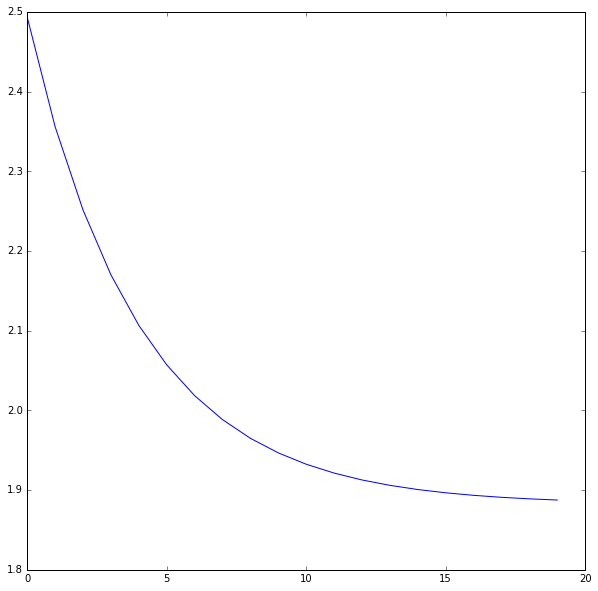
\includegraphics[scale=0.15]{2_dataloss.png}}
\subfigure[$||z_1 - W_1*a_0||^2$]{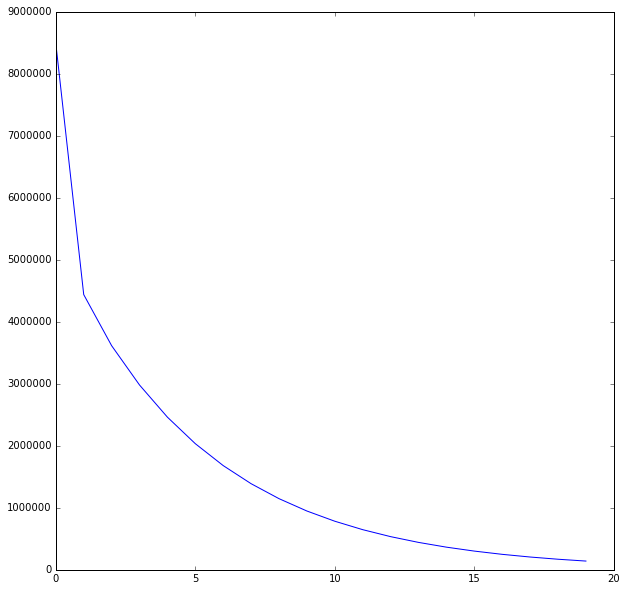
\includegraphics[scale=0.15]{2_qudraloss0-1.png}}
\subfigure[$||z_2 - W_2*a_1||^2$ ]{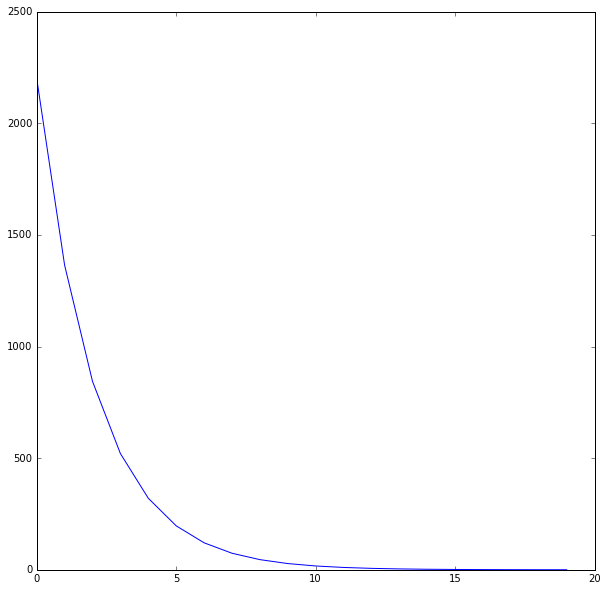
\includegraphics[scale=0.15]{2_qudraloss1-2.png}}
\caption{firt row $\epsilon$ = 0.0001, second row $\epsilon$ = 1.}
\end{figure}

\section{Update $\lambda$}
We used the same way to update $\lambda$, i.e. $\lambda \leftarrow \lambda+\beta*(z_L - W_L*a_{L-1})$.\\
As the authors explained in their answers to the review, they thought only the $z_L$ is related to the loss function. So we followed their idea but it's still unclear for us.\\
Besides, we don't understand what "quadratic decoupling" means.

\section{Bottleneck}
Until now, we don't spend any time on the efficiency of our programm because we want to make sure our implementation is correct first. But our guess is first of all, the updating for $z_L$ is most time consuming. We will try to implement Newton's method for softmax.\\
Secondly, it should be the inversing part. Because of the size of dataset, calculating the inverse or pseudo inverse is difficult even though we used the least square.\\
 
\end{document}